\chapter{Galaxy Zoo} 

O GZ é um projeto de astronomia "on-line" onde somos convidados a classificar galáxias, a ideia inicial usar a mão de obra do público em geral na pesquisa científica \cite{Raddick_2010}. Sendo hospedado em um site onde qualquer pessoa com conexão à Internet é convidada a participar da pesquisa classificando galáxias do SDSS. O projeto fez tanto sucesso que em abril de 2009, mais de 200 000 voluntários haviam feito mais de 100 milhões de classificações de galáxias. 

Podemos facilmente encontrar estes dados prontos e com uma certa facilidade no Kaggle, que é empresa subsidiária da Google LLC, é conta com uma comunidade on-line de cientistas de dados e profissionais de AM. O Kaggle permite que os usuários encontrem e publiquem conjuntos de dados, explorem e construam modelos em um ambiente de ciência de dados baseado na web, existem diversos desafios que são colocados pelo Kaggle e nosso conjunto de dados do GZ se trata de um desses conjuntos usados em um desafio. 

\begin{figure}[!ht] 
\centering 
\subfigure[ref1][Galaxias Espirais]{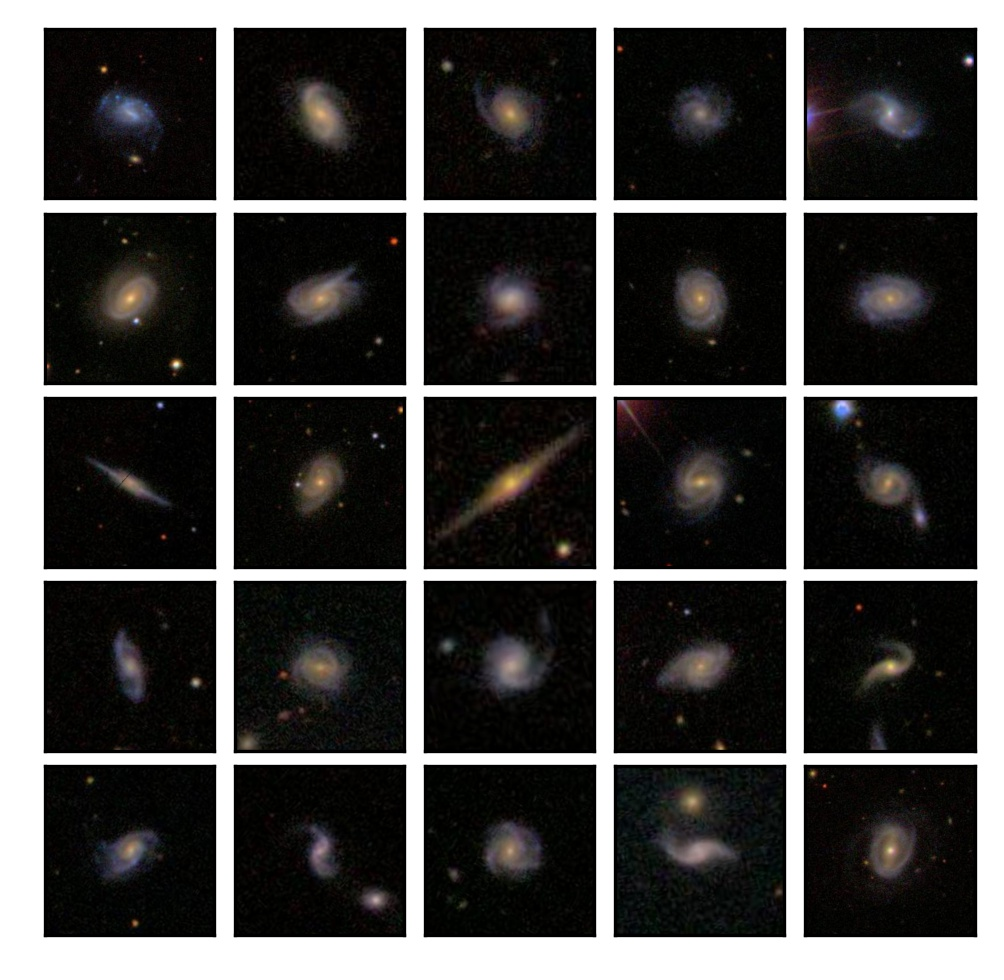
\includegraphics[width=6cm]{imagens/teste1.jpg}} 
\qquad 
\subfigure[ref2][Galaxias Elípticas]{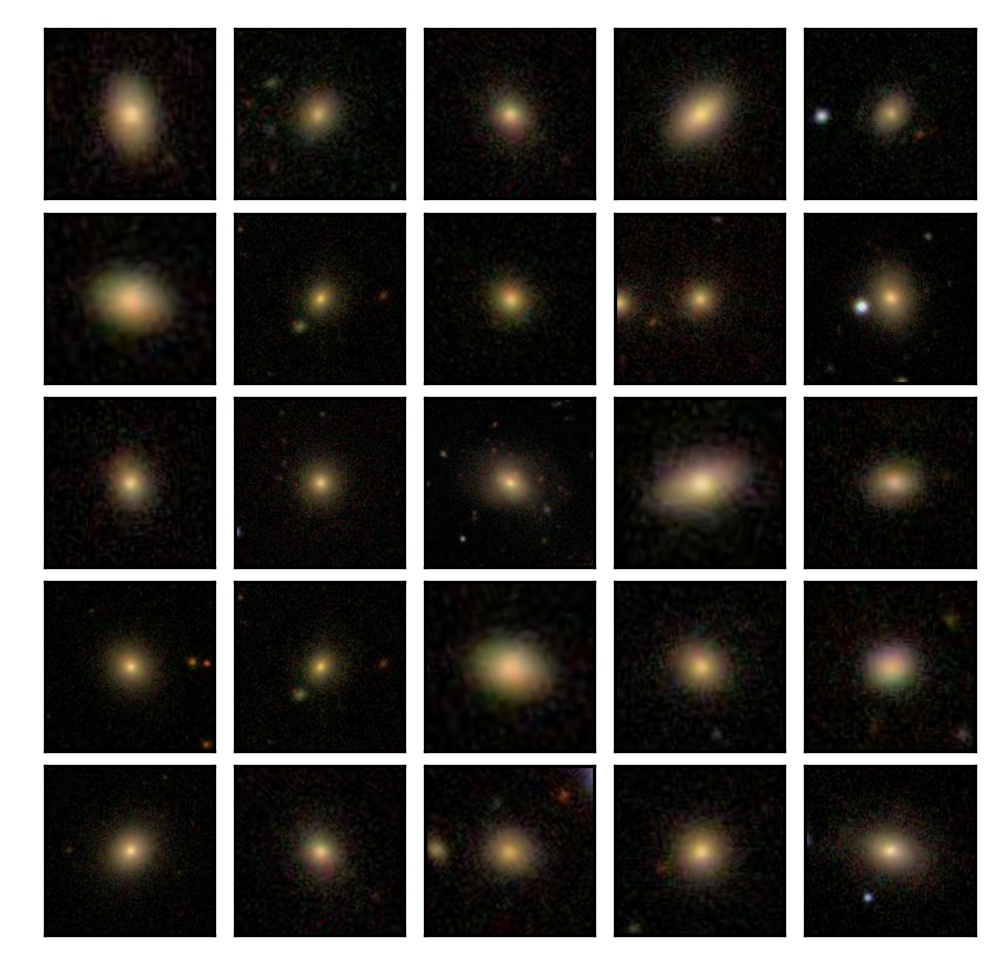
\includegraphics[width=6cm]{imagens/teste2.jpg}} 
\caption{(a) Amostra aleatória de galáxias classificadas como espirais no conjunto de dados do GZ. (b) Amostra aleatória de galáxias classificadas como elípticas no conjunto de dados do GZ.} 
\label{fig:juwdidj} 
\end{figure} 
\subsection{Descrição dos dados} 

Os dados consistem exclusivamente em imagens as quais já foram classificadas seguindo as perguntas feitas no site do GZ, temos um arquivo no formato de planilha que nos traz as informações vinculadas das imagens.  

A primeira coluna é identidades das imagens como GalaxyID, este é um ID gerado aleatoriamente que permite apenas que você combine as distribuições de probabilidade com as imagens. As próximas 37 colunas são todos números de ponto flutuante entre 0 e 1 inclusive. Estes representam a morfologia (ou forma) da galáxia em 37 categorias diferentes, conforme identificado por classificações de voluntários crowdsourced como parte do projeto GZ 2.  

Essas morfologias estão relacionadas às probabilidades de cada categoria, um número alto (próximo a 1) indica que muitos usuários identificaram esta categoria morfológica como sendo de uma galáxia com um alto nível de confiança. Números baixos para uma categoria (perto de 0) indicam que o recurso provavelmente não está presente. 

 